% !TeX spellcheck = es
\documentclass{report}
\usepackage[utf8]{inputenc}

% Títulos automáticos en español
\usepackage[spanish]{babel}

% Soporte para buenas urls e hipervínculos entre secciones
\usepackage{hyperref}

% Citas y referencias en formato APA
% Si quiere las citas y referencias en IEEE comente esta línea
\usepackage{apacite}

% Imágenes y figuras
\usepackage{graphicx}

% Código fuente con números de línea
\usepackage{listings}
% Puede cambiar el lenguaje de código fuente
% https://www.overleaf.com/learn/latex/code_listing#Supported_languages
\usepackage{multirow}


\lstset{
    language=C,
    basicstyle=\footnotesize,
    numbers=left,
    stepnumber=1,
    showstringspaces=false,
    tabsize=1,
    breaklines=true,
    breakatwhitespace=false,
}


\def \unidad{Escuela de Ingeniería en Computación}
\def \programa{Ingeniería en Computación}
\def \curso{IC6600 - Principios de Sistemas Operativos}
\def \titulo{Proyecto 2}
\def \subtitulo {Simulación de Algoritmos de Paginación}
\def \autores{
    Gerald Calderón\\
    gecalderon@estudiantec.cr\\
    2023125197\\
    
    \vspace{0.5cm}
    
    Óscar Obando\\
    osobando@estudiantec.cr\\
    2023091684
    
    \vspace{0.5cm}
    
    Samuel Zúñiga\\
    sazuniga@estudiantec.cr	\\
    2023029693
}
\def \fecha{Octubre 2025}
\def \lugar{
    San José, 
    Costa Rica
}

% Inicia el documento 
\begin{document}

% Inserta la portada del documento
\begin{titlepage}
    \begin{center}
        \vspace*{1cm}
        
        
\includegraphics[width=0.8\linewidth]{figuras/logo_tec.jpg}\\
        \LARGE
        \unidad\\
        \programa\\
        \curso
        
        \vspace{1cm}
        
        \Huge
        \textbf{\titulo}
            
        \vspace{0.5cm}
        \LARGE
        \subtitulo
            
        \vspace{1.5cm}
        
        \large    
        \autores
            
        \vfill
        
        \lugar\\
        \fecha
        
    \end{center}
\end{titlepage}

\tableofcontents

\chapter{Introducción}\label{intro}

Para este proyecto se implementó un compresor (y decompresor) de archivos de texto utilizando el algoritmo de Huffman.
Este toma un directorio con archivos de texto y los comprime en un solo archivo en binario, al descomprimir, se restaura el directorio y los archivos dentro de este.
Este sistema consiste en dos partes principales,  el programa que comprime y el programa que descomprime.
Ambos ofrecen tres modos de ejecución: serial, concurrente y paralelo.

\section {Algoritmos de Paginación}
\subsection{Óptimo}

El algoritmo óptimo de paginación es aquel que tiene la capacidad de ver el futuro, es decir, sabe cuales páginas serán utilizadas durante toda la ejecución de la máquina para poder decider a cual mandaar a memoria virtual. Su funcionamiento consiste en buscar dentro de las páginas cargadas en memoria real aquella que nunca se va a volver a utilizar o la que se va a utilizar más tarde para reemplazarla por la que se requiera cargar en dicho momento. 

Para su implementación al leer el archivo de instrucciones a utilizar se llama a la función ``parse\_for\_optimal" (ver figura \ref{fig:parse_optimal})que detecta cada aparición de ``use" o ``new" para registrar las páginas en una lista que contendrá el id de las páginas que son utilizadas en dichas instrucciones. Una vez se lee todo el archivo dicha lista de páginas es pasada al constructor de la MMU concreta que contiene el algoritmo óptimo como implementación de la función ``paging" (ver figura \ref{fig:optimal}).

\begin{figure}[h]
	\centering
	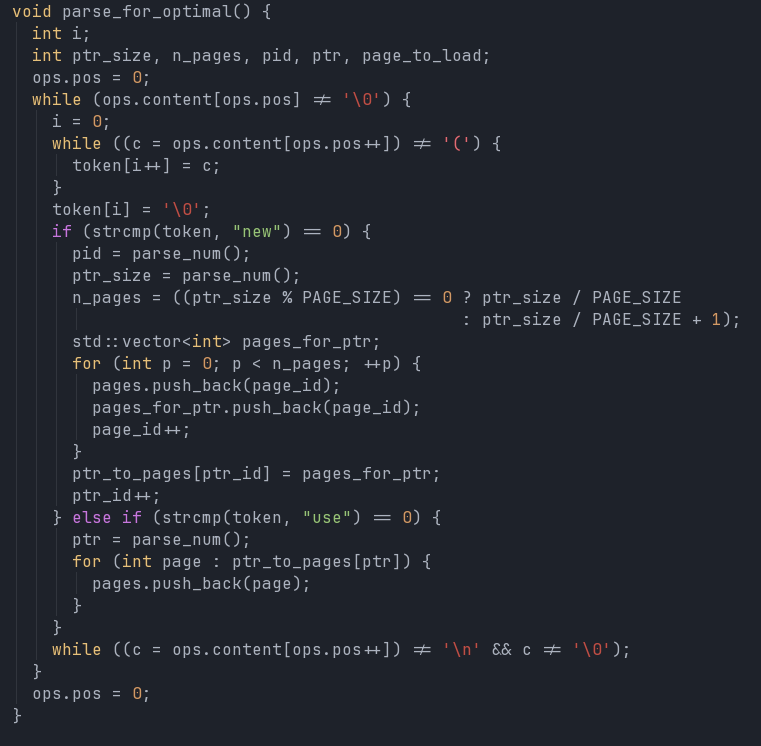
\includegraphics[width=0.8\linewidth]{figuras/parse_optimal.png}
	\caption{Ilustración de la estructura del programa}
	\label{fig:parse_optimal}
\end{figure}



\begin{figure}[h]
	\centering
	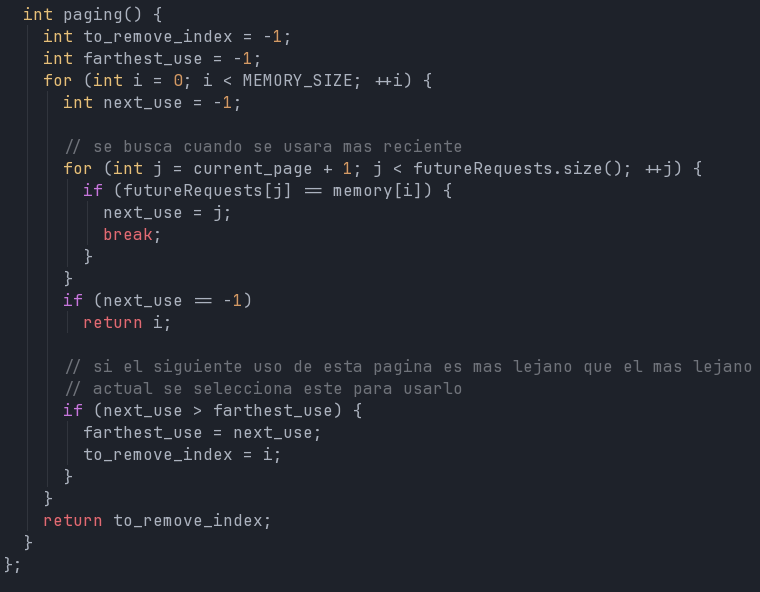
\includegraphics[width=0.8\linewidth]{figuras/optimal.png}
	\caption{Ilustración de la estructura del programa}
	\label{fig:optimal}
\end{figure}


\subsection{FIFO y Second Chance}
\subsection{LRU y MRU}
\subsection{Random}

\begin{figure}[h]
    \centering
    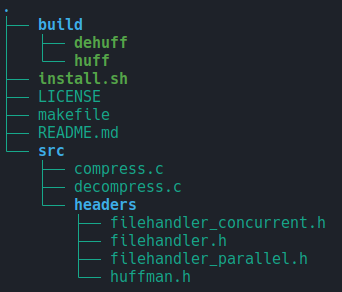
\includegraphics[width=0.8\linewidth]{figuras/estructura.png}
    \caption{Ilustración de la estructura del programa}
    \label{fig:estructura}
\end{figure}

\section{Instrucciones}
\subsubsection{Cómo instalar el programa}
\begin{enumerate}
  \item Descargue el código fuente del programa. Puede hacerlo de las dos siguientes formas:
    \begin{itemize}
      \item Dirigirse al repositorio de GitHugitb mediante su navegador a través del siguiente link: \url{https://github.com/Andres2950/PSO\_PagingSimulator.git}
      \item Instalarlo directamente con el comando \\
    \texttt{wget \url{https://github.com/Andres2950/PSO\_PagingSimulator/archive/refs/heads/main.zip}}
    \end{itemize}
  \item Descomprima el archivo .zip descargado utilizando el comando \texttt{unzip}.
  \item Al extraer el archivo podrá observar la estructura de organización similar a la figura \ref{fig:estructura}.
\item Ejecute el archivo \texttt{install.sh}, asegúrese de qué tenga permisos de ejecución, puede utilizar el comando \texttt{chmod +x install.sh} en caso de que no los posea y luego ejecute de la siguiente forma \texttt{./install.sh}. \\
  Este archivo se hará cargo de la instalación del compilador \textit{g++} necesario para compilar el código fuente. Además hará la instalación del paquete \textit{cmake} para la ejecución del archivo ``CMakeLists.txt", dicho archivo posee las instrucciones de compilación de \textit{SDL} para resolver todas las dependencias. 
\item Note que la instalación de dichos paquetes requiere permisos de usuarios root, al ejecutar el archivo \texttt{install.sh} este se volverá a ejecutar con dichos permisos, para esto solicitará la contraseña del usuario root para tener dichos permisos de ejecución (la contraseña es totalmente invisible para el programa) y así poder descargar los paquetes.
\item La compilación de los archivos se realiza sin permisos root.
%\item Además, el \texttt{install.sh} hará una copia de los binarios \texttt{huff} y \%texttt{dehuff} en el directorio \textit{/usr/bin} de la máquina para poner ser %accedidos desde cualquier lugar y utilizado en múltiples directorios sin necesidad %de mover los archivos a comprimir o descomprimir a una carpeta en particular.

\end{enumerate}

\subsection{Cómo utilizar el programa}
Una vez terminado el procedimiento de instalar el programa puede utilizar el comando \texttt{./build/app/app} en la carpeta del proyecto descargada para ejecutar el programa de simulación.

\begin{figure}[h]
    \centering
    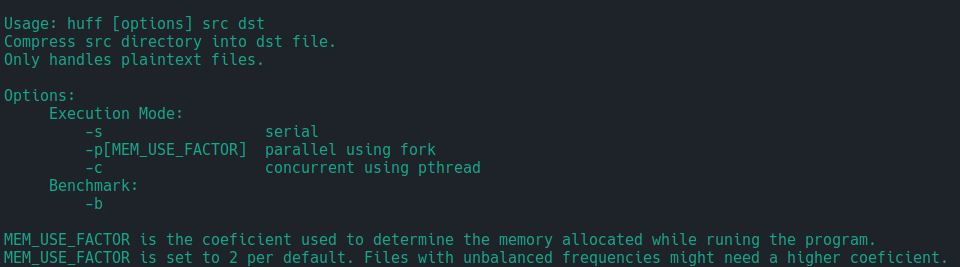
\includegraphics[width=0.8\linewidth]{figuras/huff_ayuda.png}
    \caption{Ilustración del menú de ayuda del comando huff -h}
    \label{fig:huffayuda}
\end{figure}

\begin{itemize}
  \item \textbf{huff -h}\\ \hspace{2cm}
    Provee una guía de los parámetros requeridos por el programa y su orden de entrada (Véase figura \ref{fig:huffayuda}).
  \item \textbf{huff [Opción] src dst} o \textbf{dehuff [Opción] src dst}\\
src es el directorio objetivo a ser comprimido/descomprimido\\
dst es el archivo de destino
  \item \textbf{Opciones} 
    \begin{itemize}
      \item \textbf{-s} modo de ejecución serial.
      \item \textbf{-p} modo de ejecución paralela usando fork.
      \item \textbf{-c} modo de ejecución concurrente usando pthread
      \item \textbf{-b} modo de Benchmark para comparar los tiempos de ejecuión entre los anteriores modos.
    \end{itemize}
\end{itemize}


\section{Conclusiones}
Los resultados obtenidos muestran una clara mejora en los progamas de compresión y de descompresión, a partir de esto se puede concluir que el algoritmo de Huffman implementado aprovecha mucho de las ventajas que proveen la concurrencia y paralelización. 
Esto se debe a que ambos programas manejan distintos archivos independientes entre ellos.
Esta independencia permite que los archivos puedan ser manejados por separado, sea este procesamiento por medio de hilos o de procesos hijo.
Por lo que se puede decir que cuando hay muchas subtareas independientes por hacer en un programa, es bueno considerar alguno de los dos. 

A pesar de lo dicho anteriormente, ambos en ambos modos de ejecución, ninguno se acercó al límite teórico que se propuso para cada uno.
A partir de esto se puede concluir que el overhead que produce el uso de hilos o de subprocesos no es trivial.
Al usar cualquiera de estos dos siempre es importante tomar en cuenta el overhead que estos causan para determinar si realente vale la pena usar alguna de las técnicas descritas anterormente.

Comparando los resultados que dieron las pruebas de concurrencia y las pruebas de paralelización, se puede concluir que la paralelización es ligeramente mejor que la concurrencia.
Esto se puede deber a la naturaleza de la paralelización, gracias a que cada proceso puede correr en un procesador distinto. 
También se puede deber a la necesidad de la concurrencia de cambiar de contexto frecuentemente, lo que también toma recursos de la computadora.


% Estilo de bibliografía APA
% Si quiere usar el estilo IEEE comente esta línea
\bibliographystyle{apacite}

% Descomente esta línea para usar el estilo de bibliografía IEEE
%\bibliographystyle{ieeetr}
\bibliography{referencias}

\end{document}
